\documentclass[11pt,a4paper]{article}

% Packages
%   \usepackage[english,danish]{babel}
\usepackage{fullpage}
\usepackage[english]{babel}
\usepackage[utf8]{inputenc}
\usepackage{amsmath,amscd}
\usepackage{amssymb}
\usepackage{amsthm}
\usepackage{enumerate}
\usepackage{graphicx}                    
\usepackage{framed}  
\usepackage{tikz}  
\usepackage{hyperref}  
%\usepackage{multicols}

\theoremstyle{plain}
\newtheorem{thm}{S¾tning}
\newtheorem{prop}[thm]{Proposition}
\newtheorem{lem}[thm]{Lemma}
\newtheorem{cor}[thm]{Korollar}
\newtheorem{conj}[thm]{Formodning}
\theoremstyle{definition}
\newtheorem{exercise}{Opgave}
\newtheorem{definition}[thm]{Definition}
\newtheorem{prob}[thm]{Problem}
\newtheorem{remark}[thm]{Bem¾rkning}
\newtheorem{example}[thm]{Eksempel}


% Blackboard bold
\newcommand{\NN}{\mathbb{N}}
\newcommand{\ZZ}{\mathbb{Z}}
\newcommand{\QQ}{\mathbb{Q}}
\newcommand{\RR}{\mathbb{R}}
\newcommand{\CC}{\mathbb{C}}
\newcommand{\GCD}{\operatorname{GCD}}

\title{DMFS 2023 Lectures on Graphs by Rasmus Pagh, Part 2}
%   \author{Rasmus Pagh}
\date{}

\begin{document}
	\maketitle


\section*{Litteratur}

\begin{itemize}
\item[-] CLRS~20.3 (indtil 'Properties of depth-first search' s.~567), 20.4, 20.5
\item[-] CLRS 21
\item[-] Dybde-først søgning i \emph{Noter om grafer}
\end{itemize}



\section*{Mål  % for ugen
}


\begin{itemize}
\item[-] Forståelse af algoritmer til topologisk sortering og stærke sammenhængskomponenter
\item[-] Forståelse af algoritmer til at beregne mindste udspændende træ
\end{itemize}



\section*{Plan 
%   for ugen
}

\begin{itemize}
\item[-]
%   Mandag: 
Dybde-først søgning (CLRS~20.3, indtil 'Properties of depth-first search'), topologisk sortering (CLRS 20.4).

\item[-]
%   Tirsdag: 
Mindste udspændende træer, Kruskal's og Prim's algoritmer (CLRS~21)

\item[-]
%   Fredag: 
Stærke sammenhængskomponenter (CLRS 20.5)
\end{itemize}



\section*{Opgaver}

For opgaver markeret med $\dagger$ kan du finde svar i \href{https://mitp-content-server.mit.edu/books/content/sectbyfn/books_pres_0/11599/selected-solutions.pdf}{CLRS løsningsmanual}, men det er vigtigt at du forsøger at løse opgaven, evt.~med hjælp fra din instruktor, inden du kigger dér.

%   \subsection*{Mandag}

\begin{itemize}
\item CLRS~20.3-2, 20.4-1, 20.3-12$\dagger$, 20.4-3$\dagger$

%   
%   \end{itemize}
%   
%   \subsection*{Tirsdag}
%   \begin{itemize}
%   

  \item Håndkør Kruskal's algoritme på grafen nedenfor. Overvej ved hver Union
    hvorfor kanten er 'safe'.
  \item Håndkør Prim's algoritme på grafen nedenfor. Overvej for hver tilføjet kant hvorfor den er 'safe'.
  \item CLRS~21.1-1$\dagger$, 21.1-3, 21.1-4$\dagger$, 21.2-2, 21.2-1*
\end{itemize}

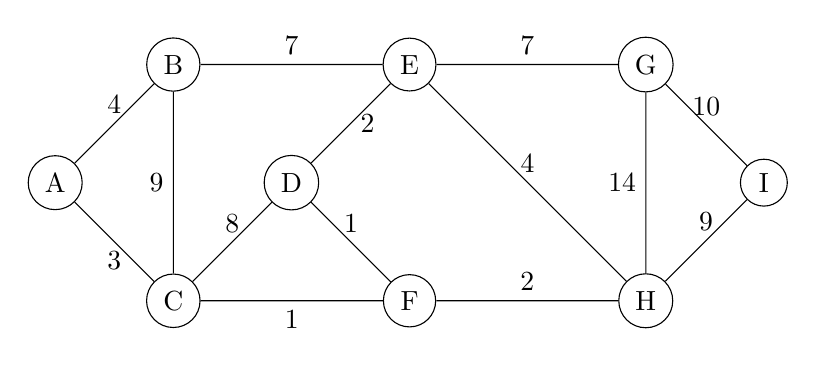
\begin{tikzpicture}[scale=1.5]
\draw 
(1, 2) node[circle, black, draw](a){A}
(2, 3) node[circle, black, draw](b){B}
(2, 1) node[circle, black, draw](c){C}
(3, 2) node[circle, black, draw](d){D}
(4, 3) node[circle, black, draw](e){E}
(4, 1) node[circle, black, draw](f){F}
(6, 3) node[circle, black, draw](g){G}
(6, 1) node[circle, black, draw](h){H}
(7, 2) node[circle, black, draw](i){I};

\draw[-] (a) -- node[above] {4} (b);
\draw[-] (a) -- node[below] {3} (c);
\draw[-] (b) -- node[left] {9} (c);
\draw[-] (c) -- node[above] {8} (d);
\draw[-] (b) -- node[above] {7} (e);
\draw[-] (c) -- node[below] {1} (f);
\draw[-] (d) -- node[right] {2} (e);
\draw[-] (d) -- node[above] {1} (f);
\draw[-] (e) -- node[above] {7} (g);
\draw[-] (e) -- node[above] {4} (h);
\draw[-] (f) -- node[above] {2} (h);
\draw[-] (g) -- node[above] {10} (i);
\draw[-] (h) -- node[left] {14} (g);
\draw[-] (h) -- node[above] {9} (i);

\end{tikzpicture}


%   \subsection*{Fredag}
\begin{itemize}
\item CLRS~20.5-2, 20.5-1, 20.5-7*
\item CLRS~problem 20-3*
\item Opgaver fra tidligere uger, som du ikke har nået at lave
\end{itemize}


\end{document}
